\documentclass[a4paper]{iacas}

\usepackage{cite}
\usepackage{hyperref}% embedding hyperlinks [must be loaded after dropping]
\usepackage{amsmath,amsthm,amssymb,amsfonts,latexsym,mathrsfs,wasysym}
\usepackage{marvosym}
\usepackage{subcaption}
\usepackage{soul,color}
\usepackage{threeparttable}% tables with footnotes
\usepackage{dcolumn}% decimal-aligned tabular math columns
\usepackage{float}
\usepackage{graphicx}
\usepackage{accents}
\usepackage{tikz}
\usepackage{lastpage}
\usepackage{fancyhdr}
\usepackage{color}
\usepackage{cancel}
\usepackage{setspace}
%\doublespacing
% or:
\onehalfspacing
%\usepackage[T1]{fontenc}
%\usepackage{bigfoot} % to allow verbatim in footnote
\usepackage[framed,numbered]{matlab-prettifier}
\pagestyle{plain}
%\usepackage[hebrew,english]{babel}
\usetikzlibrary{shapes.geometric, arrows, calc}

\newcolumntype{d}{D{.}{.}{-1}}
\graphicspath{{figures/}}

% define some commands to maintain consistency
\newcommand{\pkg}[1]{\texttt{#1}}
\newcommand{\cls}[1]{\textsf{#1}}
\newcommand{\file}[1]{\texttt{#1}}
\newcommand{\sgn}[1]{\operatorname{sgn}\left(#1\right)}
\newcommand{\sat}[1]{\operatorname{sat}\left(#1\right)}
\newcommand{\rrule}[1]{\rule[#1]{0pt}{0pt}}
\newcommand{\fracds}[2]{\frac{\displaystyle #1\rrule{-0.2em}}{\displaystyle #2\rrule{1em}}}
\newcommand{\figref}[1]{Fig.~\ref{#1}}
\newcommand{\ubar}[1]{\underaccent{\bar}{#1}}
\newcommand{\norm}[1]{\lvert \lvert \vec #1 \rvert \rvert}

%diffeomorphism

\begin{document}


\section{Calibration}

\subsection{Projection matrix computation}
The projection matrix was computed using the the DLT method:

\begin{enumerate}
\item The A matrix was built, which concentrated all the corresponding points. We have 9 points in total, which is more than required (6 pairs). Each pair can retrieve 2 unknown variables, and the camera matrix P is of size [3X4], meaning we are looking for 12 variables. The equation which has to hold is: 
\begin{equation*}
\underline{A}\underline{P} = 0
\end{equation*}
thus the problem turns into the minimization problem: $$\min\limits_{\underline{P}}||AP||_2^{2}   ; s.t. ||P||_{2}^{2}=1$$

\item Using the SVD, the A matrix was converted into [U, D, V]. P is the minimal right eigenvector. Reordering the P we obtain the original projection matrix P:

\begin{equation}
\left[
\begin{matrix}
    0.0057  &  0.0823 &  -0.0010 &  -0.8644 \\
    0.0100  & -0.0001 &   0.0820 &  -0.4891\\
   -0.0000  &  0.0000 &   0.0000 &  -0.0006
\end{matrix}
\right]
\end{equation}
\end{enumerate}



\subsection{Points reprojection, error measurement}

All the points from the 3D world coordinated were reprojected using the reprojection matrix found. To estimate the error it was decided to use the MSE method. The following table shows the reprojected coordinates for each point, and the MSE. the units of the MSE is pixels. By being around 3.5 pixels, we can assume that the error comes from the inacuracy (and inconsistency of the accuracy) of picking the points from the image manually.

%% ERRORS FIGURE

\vskip 0.1in
\begin{minipage}{\linewidth}
	\centering
	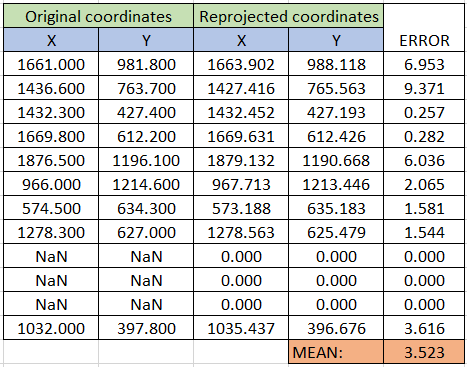
\includegraphics[scale=1]{goal_res/errors_table.png}
	\captionof{figure}{Errors of the 3D points reprojection}
	\label{fig_1}
\end{minipage}
\vskip 0.1in



\subsection{R,K matrix reconstruction}
The matrixes R, K were reconstructed using the given function. 
\newline
In this case we use the RQ decomposition, and not the QR decomposition, because we require the opposite order of the matrixes on the output. QR decomposes matrix into an orthogonal matrix and upper triangular matrix. We require the reverse order, since the K matrix, which stands first, is upper triangular, and R is an orthogonal rotation matrix:
\begin{align*}
P &= K [ R | t ] = [[KR]_{3X3} | [Kt]_{3X1} ]
\end{align*}
Why this works:
\newline
...

\subsection{Camera characteristics}
To answer this question, we normalize the camera characteristics matrix K. Knowing that the item [3,3] =1, we divide the whole matrix my this value. K obtained:

\begin{equation*}
K = 
\left[
\begin{matrix}
f_{x} & s &  x_{0}\\
0 & f_{y} & y_{0} \\
0 & 0 & 1
\end{matrix}
\right]
=
1e^{+4}
\left[
\begin{matrix}
    1.0005&    0.0070&    0.1224 \\
         0&    1.0032&   -0.1053 \\
         0&         0&    0.0001
\end{matrix}
\right]
\end{equation*}
We can see that the matrix is indeed reasonable:


\begin{enumerate}
\item The focal length values here are in the units of $[pixels]$. We can see that they are almost similar, although they differ a bit, which is okay due to inperfect camera (and other factors).
\item To obtain the focal length values in $[mm]$ as usually in cameras, we need to know the pixel size of a camera. Lets take something found over internet, some real values: "Industrial cameras usually use 1/3" sensors in case of resolutions of 640 x 480 pixels" \footnote{https://www.vision-doctor.com/en/camera-technology-basics/sensor-and-pixel-sizes.html}. Using the image provided in this source, we obtain the $[\frac{pixels}{mm}]$ value: $$m_{x} = \frac{640}{4.8} = \frac{480}{3.6} = 133.3 [\frac{pixels}{mm}]$$.
Using this on our case, finding the focal length in [mm] gives:
$$f_{x_{mm}} = \frac{f_{x}}{m_{x}} = \frac{10005}{133.3} = 75.1 [mm]$$
$$f_{y_{mm}} = \frac{f_{y}}{m_{x}} = \frac{10032}{133.3} = 75.2 [mm]$$
Which is quiet typical. 
\item We can see that the skew parameter $s$ is small relatively to $f_{x}$ and $f_{y}$, which is reasonable.
\item $x_{0}$ and $y_{0}$ indicate where the Principal Point Offset is located.
\end{enumerate}

\subsection{Orientation of the camera}
We perform the sanity check. We know that in the Camera coordinates, the Y direction approximately lies on the Z direction of the World coordinates. R matrix rotates from World to Camera. Thus, we obtain:

\begin{equation*}
\left[
\begin{matrix}
0\\
0 \\
1
\end{matrix}
\right]
\left[
\begin{matrix}
    0.1897  &  0.9816  & -0.0216\\
    0.0189  &  0.0183  &  0.9997\\
   -0.9817  &  0.1900  &  0.0151
\end{matrix}
\right]
= 
\left[
\begin{matrix}
   -0.0216\\
    0.9997\\
    0.0151
\end{matrix}
\right]
\end{equation*}

Thus, we indeed see that the rotation matrix is reasonable and that Z direction in World changed to Y direction in Camera coordinate system.


\subsection{Translation vector}
In the calculated P matrix, the derived translation vector is indeed in the Camera coordinates. We translate it into the the World coordinates using the given equation: $$t_{C} = -Rc$$, where $c$ is the translation in the World space. The derived c is:

\begin{equation*}
c = -R^{T}t = 
\left[
\begin{matrix}
-66.66\\
15.3\\
14.13
\end{matrix}
\right] [m]
\end{equation*}

Everything is in meters. And indeed, we need apply this transformation to move from Camera Origin to the World Origin in the world coordinates.

\subsection{Camera plotting}
The camera location is being plotted onto the existing Figure. We have used the same translation vector that was found in the previous subsection, this is actually the camera location.


\vskip 0.1in
\begin{minipage}{\linewidth}
	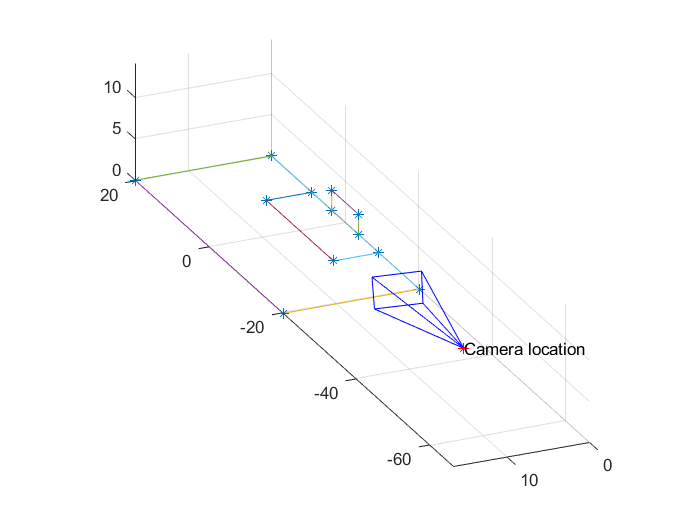
\includegraphics[scale=0.8]{goal_res/camera_loc.png}
	\captionof{figure}{Camera location and camera frame}
	\label{fig_2}
\end{minipage}
\vskip 0.1in


\subsection{Goal detection}
Using \textbf{only} the above information, it is impossible to determine whether the ball has crossed the line. There is ambiguity the distance of the ball from the camera. We can only project the vector, on which the ball can be placed in the real world:

\vskip 0.1in
\begin{minipage}{\linewidth}
	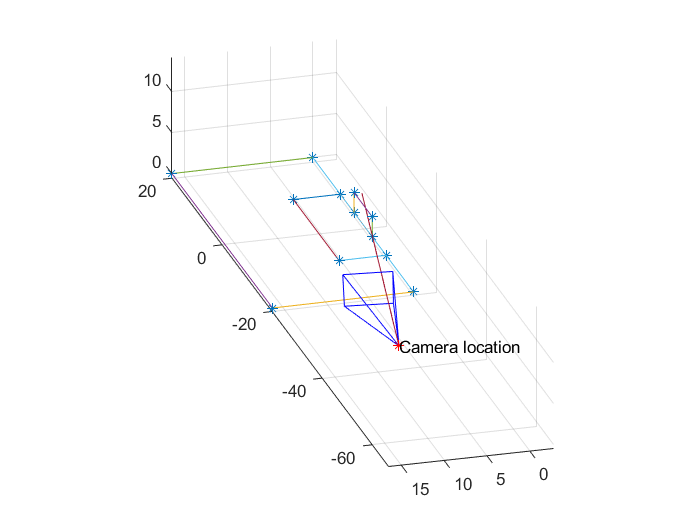
\includegraphics[scale=0.8]{goal_res/goal_camera_frame.png}
	\captionof{figure}{Projection of the vector where the ball is placed}
	\label{fig_3}
\end{minipage}
\vskip 0.1in

We need aditional information to determine the distance of the ball. This information can be the size of the ball, to determine at which distance the ball will take indeed as many pixels as it takes in the picture. This is out of the scope of this question, thus will not be done here. 



%\begin{equation*}
%\end{equation*}




\section{Depth with Stereo}



\end{document}




















